\documentclass[11pt,french]{article}
\usepackage[T1]{fontenc}
\usepackage[utf8]{luainputenc}
\usepackage{graphicx}
\usepackage{babel}
\usepackage[top=2cm, bottom=2cm, left=2.5cm, right=2.5cm]{geometry}
%Gummi|065|=)
\title{\textbf{Rapport d'activit\'e 2012-2014}}
\author{Laurent Mirabito}
\date{}
\begin{document}

\maketitle

\section*{D\'eveloppement d'un prototype technologique de calorim\`etre hadronique semi-digitale}

Le groupe ILC de l'IPN Lyon a d\'ebut\'e en 2010 la construction d'un prototype de
calorim\`etre hadronique Semi Digital (SDHCAL) constitu\'e de 50 chambres \`a plaques r\'esistives en verre (GRPC) de 1 m$^2$ intercal\'ees entre 50 plans de 2.8 cm d'absorbeur d'acier. 
Chaque chambre GRPC est \'equip\'ee d'un plan de damiers d'un cm2 connect\'es \`a des ASICs de type
HARDROC du groupe OMEGA du LAL contrôl\'es et lus par des cartes (DIF) d\'edi\'ees d\'evelopp\'ees au LAPP.

Ce prototype, dont l'assemblage s'est termin\'e en 2011, a fait l'objet de plusieurs campagnes de tests sur faisceaux en 2011, 2012 et finalement 2014. Le d\'etecteur a \'et\'e expos\'e à des faisceaux de pions et d'\'electrons de 10 \`a 90 GeV/c. Mon travail dans ce cadre a \'et\'e d'une part de d\'evelopper les syst\`emes d'acquisition et de monitorage de donn\'ees et d'autre part la reconstruction et l'analyse des amas hadroniques dans le calorim\`etre.

\subsection*{Syst\`eme d'acquisition}
Le syst\`eme d'acquisition initialement pr\'evu en 2011 \'etait bas\'e sur un bus bidirectionnel autorisant l'envoi de l'horloge et de commandes (trigger,reset...) dans un sens et la collecte des donn\'ees et des v\'etos dans l'autre. Des probl\`emes dans l'int\'egrit\'e des donn\'ees collect\'ees nous ont amen\'e en 2012 \`a s\'eparer ces deux fonctions et \`a utiliser un bus USB de d\'everminage implant\'e sur la carte DIF pour la lecture des donn\'ees. L'ensemble des tests de 2012 ont \'et\'e r\'ealis\'es avec cette architecture. N\'eanmoins ce bus est de faible bande passante ($\le$ 10 Mbit/s) et contribue significativement au temps mort lors des prises de donn\'ees. Le d\'eveloppement en lieu et place  d'un adapteur USB2 (80 Mbit/s) nous a permis en 2014 d'am\'eliorer l'efficacit\'e d'acquisition de 7 a 20 \% et donc la statistique de donn\'ees collect\'ees. Une autre am\'elioration importante du point de vue de la fiabilit\'e et de la portabilit\'e a \'et\'e le remplacement des 6 ordinateurs PC connect\'es \`a 22 Hub USB par des micro ordinateurs raspberry pi equip\'es de hub 12 ports d\'evelopp\'es \`a l'institut (figure \ref{rpi}). Ces micro ordinateurs, bas\'es sur des processeurs de t\'el\'ephone portable, sont \'economiques, de petites taille et de tr\`es basse consommation. Un processeur pour 4 chambres a ainsi pu \^etre accroch\'e au prototype optimisant d'une part le cablage et la manutention du d\'etecteur mais \'egalement les performances de la lecture des bus USB du fait du nombre r\'eduit de cartes d'acquisition vu par chaque ordinateur. Cependant l'architecture de ces processeurs (ARM) diff\`ere de celle des PCs standards et  l'environnement logiciel de CMS (XDAQ) utilis\'e jusqu'alors n'est pas disponible pour ceux-ci. J'ai d\^u par cons\'equent r\'e\'ecrire un syst\`eme d'acquistion complet bas\'e d\'esormais sur DIM (environnement logiciel de l'exp\'erience DELPHI). Cette nouvelle version de l'acquisition plus portable et plus l\'eg\`ere en terme d'installation a \'et\'e utilis\'ee sur tous les tests et mesures de 2013 et 2014 pr\'esent\'es ci-dessous. L'architecture et les performances sont d\'ecrites dans une note technique de CALICE sur le prototype SDHCAL en cours de r\'edaction.       
\begin{figure}
\centerline{\rotatebox{180}{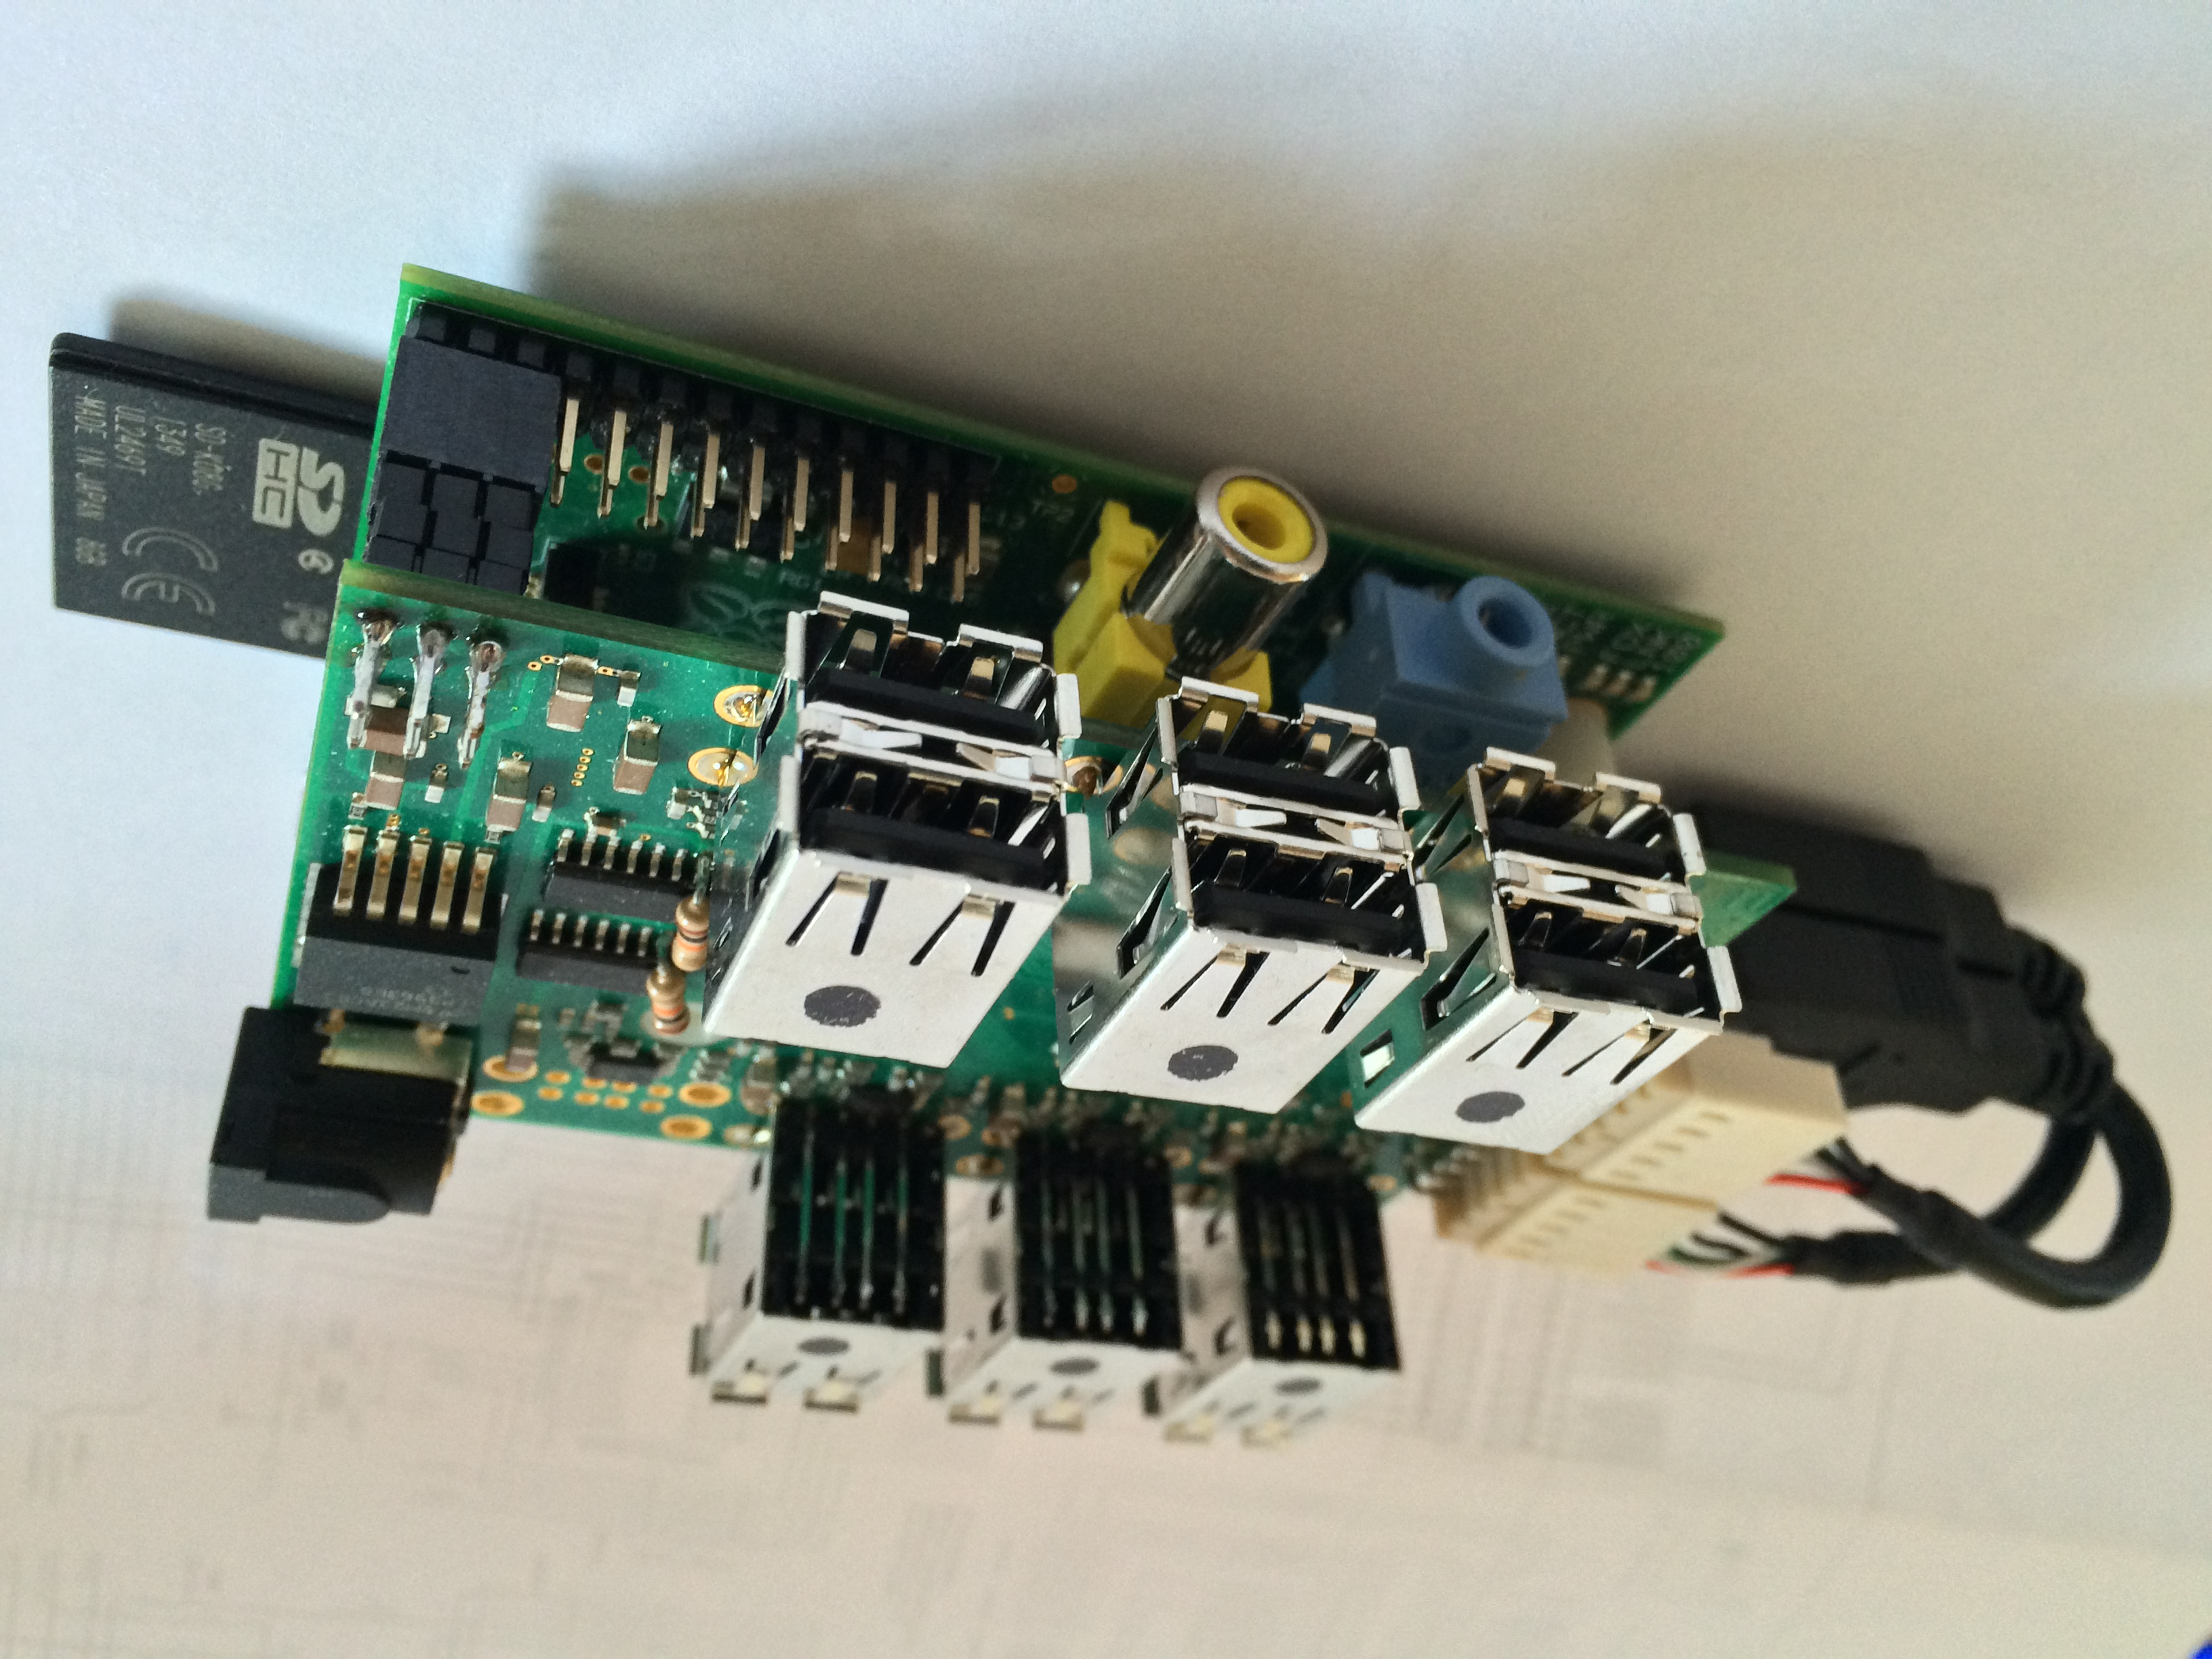
\includegraphics[height=0.4\textheight]{./rpi.JPG}}}
\caption{Micro ordinateur raspberry pi \'equip\'e d'un hub USB d\'evelopp\'e \`a l'IPNL }
\label{rpi}
\end{figure}
\subsection*{Reconstruction des gerbes hadroniques}

Outre les programmes d'\'ecriture et de pr\'efiltrage de donn\'ees en temps que j'ai d\'evelopp\'e, j'ai \'egalement particip\'e \`a l'analyse des \'echantillons. Les deux points sur lesquels j'ai plus particuli\`erement contribu\'e sont d'une part l'\'etude de la topologie des \'evenements et d'autre part celle de la r\'esolution en \'energie. L'utilisation des calculs d'axes principaux des gerbes permet d'\'eliminer facilement la contamination de muons issus de faisceau ou de gerbe cosmique. La reconstruction d'\'el\'ement de traces \`a l'aide de technique de transform\'ee de Hough ou combinatoire permet d' \'eliminer les gerbes d'\'electrons contaminant l'\'echantillon. Ces caract\'eristiques topologiques sont ensuite utilis\'ees, combin\'ees avec les informations semi digitales, pour am\'eliorer la r\'esolution en \'energie (comptage des hits, passant les 3 seuils). On obtient une r\'esolution comparable \`a celle obtenue dans la collaboration CALICE par le calorim\`etre hadronique analogique ($\simeq 7 \% $  pour des pions de 80 GeV). Ces r\'esultats ont fait l'objet d'une note d'analyse CALICE \cite{can37}.   
      
\section*{ Application des chambres GRPC \`a la tomographie muonique des volcans (TOMUVOL)}

L'exp\'erience TOMUVOL est un projet  de tomographie de volcan \`a l'aide de muons atmosph\'eriques commun \`a des laboratoires de l'IN2P3 (LPC et IPNL) et de l'INSU (LMV). En positionant un d\'etecteur \`a flan de volcan et en enregistrant l'incidence des muons le traversant on obtient une mesure de  l'att\'enuation du flux qui d\'epend  de la densit\'e des roches travers\'ees. Cette mesure, combin\'ee \`a des mesures plus classiques de vulcanologie, permet de dresser une cartographie densitom\`etrique pr\'ecise des volcans.

La possibilit\'e de construire des d\'etecteurs de grande tailles, robustes, \`a faible co\^ut, et d'une pr\'ecison g\'eom\`etrique suffisante fait des GRPC des candidats int\`eressants pour cette mesure. Un premier t\'elescope constitu\'e de 2 chambres de 1 m$^2$ et d'une petite chambre de 0.16 m$^2$, a permis de valider ce concept lors de deux campagnes de prises de donn\'ees au Puy de D\^ome en 2011 et 2012. Ces donn\'ees ont fait l'objet d'une publication \cite{gid}.  Notre contribution,\`a ce niveau du projet a \'et\'e essentielle puisque nous avons install\'e la quasi totalit\'e  de l'appareillage exp\'erimental, et fourni les outils logiciels pour l'utiliser et analyser les donn\'ees.

Depuis 2013, un prototype plus r\'ealiste de t\'elescope constitu\'e de 4 plans de 6 chambres de 0.16 m$^2$ a \'et\'e assembl\'e sous la maitrise d'oeuvre du LPC. Ma participation a principalement consist\'e en la mise \`a jour du syst\`eme d'acquisition du t\'elescope et des stations de tests des chambres ainsi qu'un support \`a la mise en oeuvre des prises de donn\'ees. Une nouvelle campagne de mesures vient de se terminer et un article est en cours de r\'edaction.

Plusieurs d\'eveloppements int\'eressants restent ouverts. Il faut d'abord "tropicaliser" le d\'etecteur pour le rendre autonome sur de longues p\'eriodes dans des conditions climatiques vari\'ees (syst\`eme de s\^uret\'e ,ajustement des consommations \'electrique, des flux de donn\'ees...). D'autre part un certain nombre d'am\'eliorations sont envisageables, entre autres l'augmentation du nombre de plans en utilisant une \'electronique \`a pistes, ou la mesure des temps de vols pour minimiser le bruit de fond.      

\section*{Utilisation de chambres GRPC pour la mise \`a niveau du syst\`eme de chambre a muons de CMS}

D\'ebut 2012, un test sur un faisceau de haute intensit\'e de chambres GRPC constitu\'ees de verre dop\'e de faible r\'esistivit\'e ( $ \simeq 10^{11} \Omega.cm) $ a d\'emontr\'e la stabilit\'e de collection de ces GRPC jusqu'\`a des flux de 10 kHz/cm$^2$ d'\'electron de 6 GeV \cite{desy}. Il a alors \'et\'e possible de proposer ces chambres comme une alternative aux chambres GEM pour \'equiper les stations avant de d\'etection de muons dans CMS lors de la mise \`a niveau de seconde phase en 2023. Lors de ces deux derni\`eres ann\'ees nous avons valid\'e ces d\'etecteurs lors de deux tests suppl\'ementaires. Quatres d\'etecteurs de 900 cm$^2$ equip\'es de chambres en verre dop\'e ont \'et\'e expos\'es \`a un haut flux de $\gamma$ au GIF au CERN durant plus de six mois, l'efficacit\'e de d\'etection de muons cosmiques \'etant continuellement contr\^ol\'ee. La stabilit\'e de l'efficacit\'e de d\'etection a \'et\'e confirm\'ee mais plusieurs probl\`emes dans les syst\`emes de gaz, de haute tension ou dans la construction des chambres nous am\`ene \`a r\'ep\'eter cette mesure en 2015 sur la nouvelle facilit\'e d'irradiation du CERN (GIF++) avant de pouvoir publier ces r\'esultats. Un second test au mois d'ao\^ut 2014 sur un faisceau de pion de basse \'energie a confirm\'e les mesures du test \`a DESY. Il nous a permis de tester ces chambres dans une configuration plus proche de celle envisag\'ee pour CMS: au lieu d'un plan damiers collectant les charges d'une chambre, un circuit imprim\'e grav\'e de 128 pistes sur ces deux faces collecte les charges de deux chambres simultan\'ement. La lecture des pistes \'etait r\'ealis\'ee par les m\^emes chips HardRoc2. Les pistes \'etaient \'egalement lues par groupe de 64 de mani\'ere analogique \`a l'autre extr\'emit\'e et un TDC d\'evelopp\'e par le groupe \'electronique de l'IPNL \'etait impl\'ement\'e dans le FPGA de la carte de lecture afin de tester les capacit\'es  de mesure de temps des d\'etecteurs. Plusieurs d\'eveloppements (chambres multigap, TDC, utilisation de chips PETIROC d\'evelopp\'e par Omega) sont en cours pour proposer une mesure pr\'ecise ($\le$ 50 ps) du temps dans ces chambres. Outre une r\'eduction massive du bruit de fond combinatoire entre les stations de mesures, cela permettrait une mesure pr\'ecise de la coordonn\'ee transverse.            

\section*{Algorithmes de reconstruction de traces rapides pour le d\'eclenchement de premier niveau de CMS} 

La mise \`a niveau  de phase 2 du trajectographe silicium de CMS pr\'evoit d'inclure des traces de haute impulsion transverse dans le syst\`eme de d\'ecision du d\'eclenchement de premier niveau. Ceci implique de fortes contraintes de conception et de performance en temps ($< ~ 10 \mu s$ ) dans un environnement fortement bruit\'e, l'empilement de collisions \'etant typiquement de 140 par croisement de faisceau. La solution choisie est l'assemblage de Pt-modules constitu\'es de deux senseurs de silicium s\'epar\'es de 2 mm, l'angle de travers\'ee du module est calcul\'e dans l'electronique embarqu\'ee et un germe est renvoy\'e au syst\`eme d\'eclenchement  \`a chaque croisement de faisceau si cet angle est compatible avec un Pt$>$ 2 GeV/c. N\'eanmoins la contamination en germes non issus de traces de haut Pt reste \'elev\'ee et la reconstruction rapide des traces ardue. Plusieurs approches sont actuellement \'etudi\'ees. L'une d'elle est la reconstruction compl\`ete des traces en paral\`elle sur de nombreux FPGA. Nous avons d\'ecid\'e d'adopter une approche hybride en utilisant des asics d\'edi\'es de m\'emoires associatives dans lesquelles les motifs de traces traversant un secteur donn\'e du trajectographe sont stock\'es et compar\'es au germe provenant de chaque collision. Cet asic, originellement d\'evelopp\'e pour la reconstruction en ligne des traces de CDF, a \'et\'e am\'elior\'e pour \^etre utilis\'e dans le Fast TracKer d'ATLAS (Niveau 2 du d\'eclenchement). A l'issue de cette reconaissance de motifs, le filtrage est fortement
am\'elior\'e et jusqu'\`a 70 \% des germes s\'electionn\'es sont issus de traces de haut Pt. Il reste cependant \`a reconstruire et \`a ajuster ces traces en minimisant le taux de fant\^omes. Le groupe de Lyon s'est concentr\'e sur la simulation de l'asic et l'optimisation des banques de motifs inclut dans la simulation du trajectographe ainsi que sur les algorithmes de reconstruction de trace (apr\`es filtrage) impl\'ementables dans des FPGA. J'ai particuli\`erement d\'evelopp\'e un filtre bas\'e sur la transform\'ee de Hough dont j'ai v\'erifi\'e les performances en mode paral\`elle en le portant sur un processeur graphique (GPU Nvidia). Cet algorithme a ensuite \'etait inclus dans la reconstruction officielle de CMS. La figure \ref{track} montre l'efficacit\'e de reconstruction des traces apr\`es le filtrage par les m\'emoires associatives et la reconstruction. Une note technique est en cours de r\'edaction pour d\'ecrire l'ensemble des processus de filtrage.
\begin{figure}
\centerline{{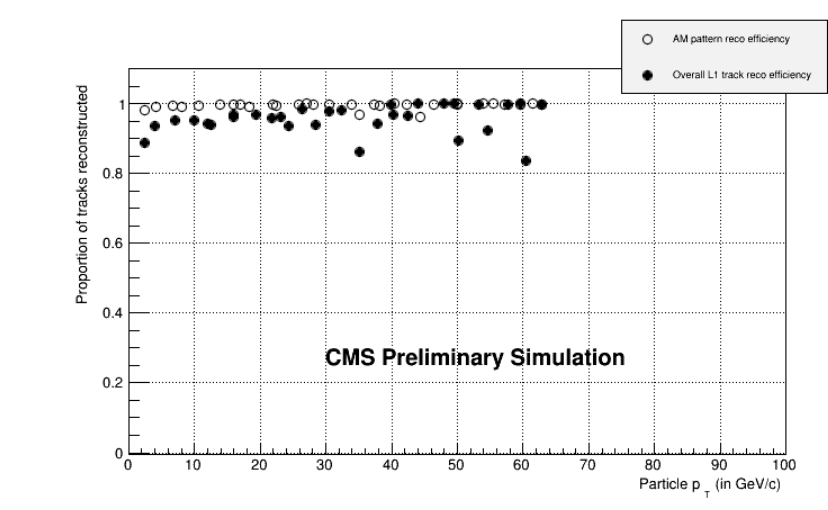
\includegraphics[height=0.4\textheight]{./TrackEff.png}}}
\caption{Efficacit\'e de reconstruction des traces en fonction de l'impulsion transverse, apr\`es l'\'etape de m\'emoire associative et apr\'es la reconstruction compl\`ete; les traces sont issues d'\'ev\`enements 4-top dans un empilement de 140 collisions}
\label{track}
\end{figure}


En 2014 nous avons obtenu, conjointement avec le groupe ATLAS du LPNHE, un financement de l'ANR pour le d\'eveloppement d'un nouvel asic de m\'emoire associative et d'un banc test de d\'emonstration des performances de reconstruction de traces combinant cet asic et les algorithmes de filtrages cod\'es sur FPGA. Un ing\'enieur \'electronicien a \'et\'e embauch\'e en CDD et travaille actuellement sur la mise au point de ce test.

\section*{Perspectives}

En 2015 une derni\`ere campagne de prises de donn\'ees avec le prototype SDHCAL devrait permettre de finaliser les analyses de gerbes hadroniques, les simulations actuelles ne reproduisant pas compl\`etement le profil des gerbes \`a haute \'energie. Un test combin\'e des calorim\`etre electromagn\'etique et hadronique est \'egalement pr\'evu. Un dernier d\'eveloppement est la r\'ealisation de chambre GRPC de plus grande taille (2 et 3 m$^2$) n\'ecessaire pour valider l'architecture des modules pr\'evue dans l'ILD. Ces chambres seront \'equip\'es d'une nouvelle \'electronique et de nouvelle carte d'acquisition. Je devrais \^etre fortement impliqu\'e dans la mise au point du syst\`eme de lecture.

Je devrais \'egalement particip\'e \`a la construction de chambres GRPC \`a verre dop\'e de grande taille \'equip\'ees d'une nouvelle \'electronique permettant la mesure pr\'ecise des temps de vols. De nouveau le syst\`eme de lecture est \`a d\'evelopper et pourrait \^etre bas\'e sur les liens rapides (GBT) pr\'evus dans la mise a niveau phase 2 de CMS.

Enfin, tout en continuant mes \'etudes sur les algorithmes de reconstruction de traces impl\'ementables sur FPGA, je pense m'impliquer davantage dans la r\'ealisation et l'op\'eration du banc test de d\'eclenchement utilisant les m\'emoires associatives. 
                  
\begin{thebibliography}{2}
   \bibitem[1]{can37} CALICE collaboration analysis note 037, 2014 
   \bibitem[2]{gid} {\it Towards a muon radiography of the Puy de Dôme} - C. Cârloganu, V. Niess, S. Béné, E. Busato, P. Dupieux, F. Fehr, P. Gay, D. Miallier, B. Vulpescu, P. Boivin, C. Combaret, P. Labazuy, I. Laktineh, J.-F. Lénat, L. Mirabito, and A. Portal; 2012; GID Volume2, Number 2 Page(s) 765-780.L. LAMPORT, 
   \bibitem[3]{desy}{\it High-rate glass resistive plate chambers for LHC muon detectors upgrade}
  I.~Laktineh, L.~Caponetto, S.~Cauwenbergh, C.~Combaret, I.~Crotty, Y.~Haddad, G.~Grenier and R.~Guida {\it et al.}. 10.1109/NSSMIC.2012

\end{thebibliography}

\end{document}
